\chapter{Eletronegatividade, polaridade e forças intermoleculares}\label{ch:g11:polarity-and-cohesion}

Uma lagartixa sobe pelo vidro de uma janela e fica pendurada nele por um
único dedo, sem cola nem ventosa. Uma \omterm{def:g7:atoms-and-molecules:molecule}{molécula} de água, \ce{H2O}, é mais
leve que uma \omterm{def:g7:atoms-and-molecules:molecule}{molécula} de sulfeto de hidrogênio, \ce{H2S}, mas a água
ferve a \qty{100}{\celsius}, enquanto o sulfeto de hidrogênio é um gás
até \qty{-60}{\celsius}. As duas histórias falam da mesma coisa: as
forças que prendem as \omterm{def:g7:atoms-and-molecules:molecule}{moléculas} umas às outras, e a outras coisas. Elas
são muito mais fracas que as \omterm{def:g10:lewis-and-shape:covalent-bond}{ligações covalentes} dentro de uma \omterm{def:g7:atoms-and-molecules:molecule}{molécula},
mas decidem se uma substância é um gás, um líquido ou um sólido à
temperatura ambiente, e se uma lagartixa cai.

\begin{recall}
Uma \omterm{def:g10:lewis-and-shape:covalent-bond}{ligação covalente} é um par de \omterm{def:g9:inside-the-atom:nucleus}{elétrons} compartilhado por dois
\omterm{def:g7:atoms-and-molecules:atom}{átomos}; as \omterm{def:g10:lewis-and-shape:lewis-structure}{estruturas de Lewis} mostram os \omterm{def:g10:lewis-and-shape:lone-pair}{pares ligantes} e os \omterm{def:g10:lewis-and-shape:lone-pair}{pares não
ligantes}, e os pares em volta de um \omterm{def:g7:atoms-and-molecules:atom}{átomo} central decidem a geometria de
uma \omterm{def:g7:atoms-and-molecules:molecule}{molécula} (\cref{ch:g10:lewis-and-shape}). Os \omterm{def:g9:ions:ion}{íons} têm carga; num
sólido iônico, os \omterm{def:g9:ions:ion}{íons} positivos e negativos se atraem
(\cref{ch:g9:ions}).
\end{recall}

\begin{omfigure}
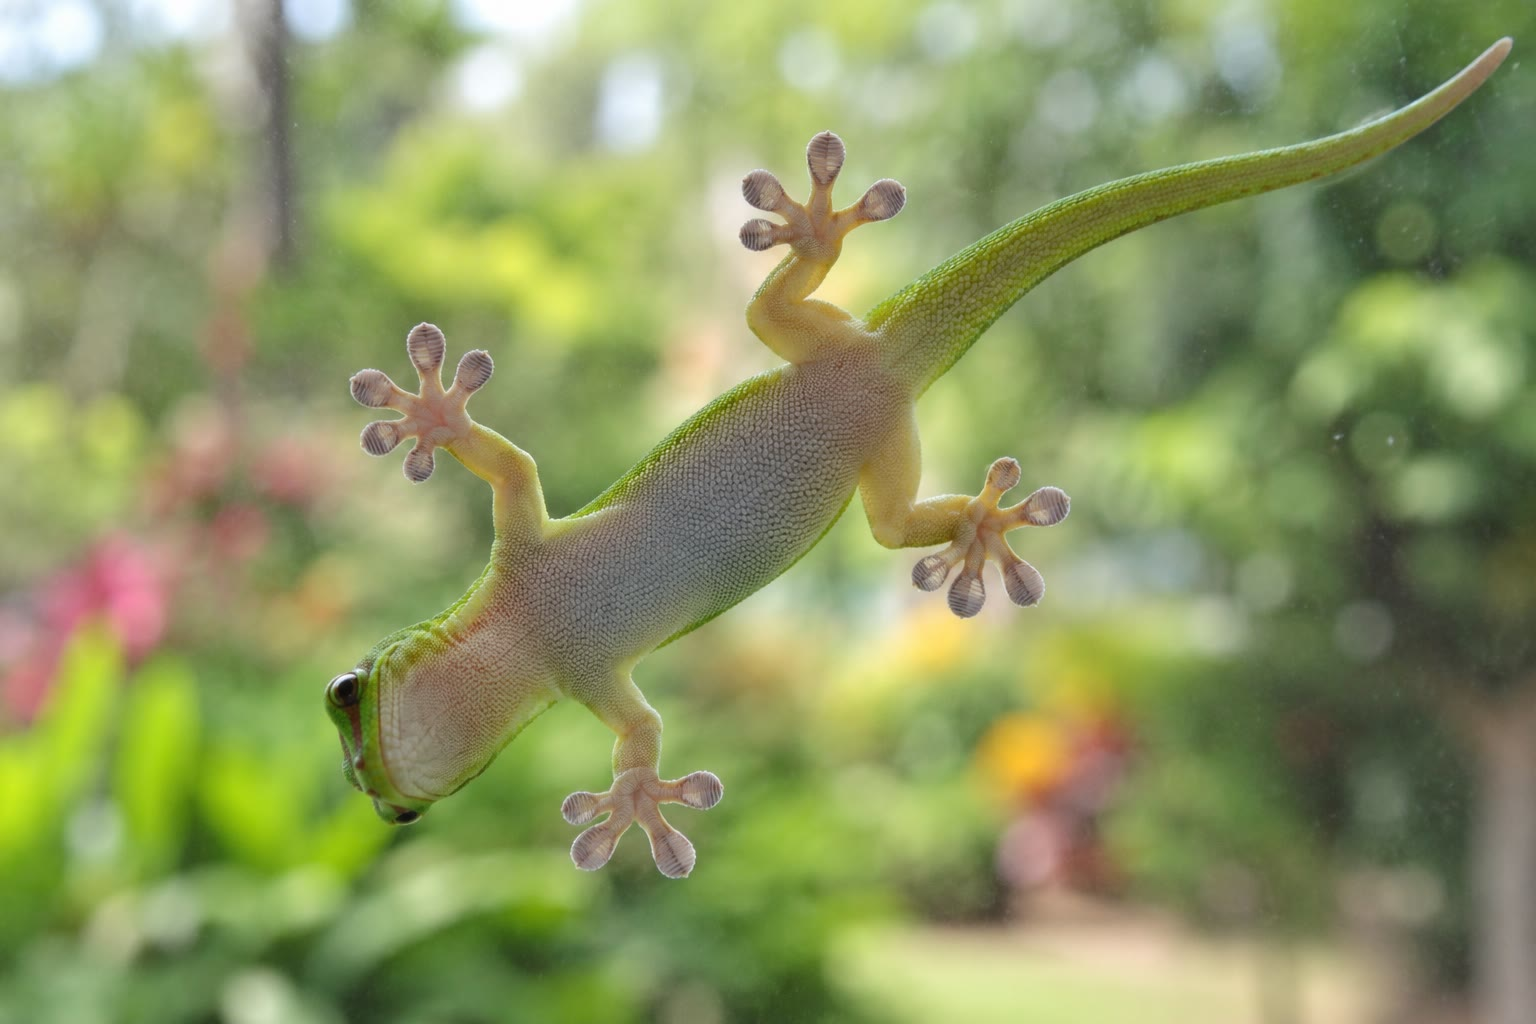
\includegraphics[width=0.5\linewidth]{images/book1/ai/g11-gecko-glass.jpg}

{\small Uma lagartixa num vidro: as almofadinhas dos seus dedos se
prendem por forças entre \omterm{def:g7:atoms-and-molecules:molecule}{moléculas}.}
\end{omfigure}

\section{A eletronegatividade}

\begin{definition}[Eletronegatividade]\label{def:g11:polarity-and-cohesion:electronegativity}
A \emph{eletronegatividade}\index{eletronegatividade} de um elemento
mede com que intensidade os seus \omterm{def:g7:atoms-and-molecules:atom}{átomos}, numa \omterm{def:g7:atoms-and-molecules:molecule}{molécula}, atraem os
\omterm{def:g9:inside-the-atom:nucleus}{elétrons} das ligações que compartilham. É um número sem unidade; na
escala usual, ele vai de cerca de 0.8 a cerca de 4.
\end{definition}

\begin{omfigure}
% ledger: en:H, en:Li, en:Be, en:B, en:C, en:N, en:O, en:F, en:Na, en:Mg, en:Al, en:Si, en:P, en:S, en:Cl, en:K, en:Ca
\omperiodictable[upto=20, f block=false, cell=0.9cm, values={H/2.20,
  Li/0.98, Be/1.57, B/2.04, C/2.55, N/3.04, O/3.44, F/3.98, Na/0.93,
  Mg/1.31, Al/1.61, Si/1.90, P/2.19, S/2.58, Cl/3.16, K/0.82, Ca/1.00},
  highlight={F,O,N,Cl}]

{\small \omterm{def:g11:polarity-and-cohesion:electronegativity}{Eletronegatividades} dos vinte primeiros elementos (escala de
Pauling; nenhum valor é dado para o hélio, o neônio e o argônio, que aqui
não formam ligações). Em destaque: os quatro mais eletronegativos.}
\end{omfigure}

\begin{proposition}[Tendências na tabela]\label{prop:g11:polarity-and-cohesion:trends}
% ledger: en:F, en:Li, en:Cl, en:K
A \omterm{def:g11:polarity-and-cohesion:electronegativity}{eletronegatividade} aumenta da esquerda para a direita ao longo de um
período e diminui de cima para baixo num grupo. O flúor (3.98) é o
elemento mais eletronegativo; os \omterm{def:g10:electron-shells:family}{metais alcalinos} são os menos
eletronegativos (lítio 0.98, potássio 0.82).
\end{proposition}

\begin{proof}
Leitura da tabela: ao longo do período 2, $0.98 < 1.57 < 2.04 < 2.55 < 3.04 <
3.44 < 3.98$; descendo o \omterm{def:g9:periodic-table-first-look:period}{grupo} 17, o flúor, $3.98$, está acima do cloro,
$3.16$; descendo o \omterm{def:g9:periodic-table-first-look:period}{grupo} 1, $2.20$, $0.98$, $0.93$, $0.82$. (Por que é
assim é explicado no volume do primeiro ano da universidade.)
\end{proof}

\begin{history}[A escala de Pauling, 1932]
O químico Linus Pauling construiu a primeira escala de
\omterm{def:g11:polarity-and-cohesion:electronegativity}{eletronegatividade} em 1932, a partir das energias das ligações entre
\omterm{def:g7:atoms-and-molecules:atom}{átomos} diferentes. Ele deu ao flúor o maior valor, e a escala usada
neste capítulo ainda leva o seu nome.
\end{history}

\section{Ligações polares e moléculas polares}

\begin{definition}[Ligação polar, carga parcial]\label{def:g11:polarity-and-cohesion:polar-bond}
Uma \omterm{def:g10:lewis-and-shape:covalent-bond}{ligação covalente} entre dois \omterm{def:g7:atoms-and-molecules:atom}{átomos} de \omterm{def:g11:polarity-and-cohesion:electronegativity}{eletronegatividades} diferentes
é uma \emph{ligação polar}\index{ligacao polar@ligação polar}: o par compartilhado fica
mais perto do \omterm{def:g7:atoms-and-molecules:atom}{átomo} mais eletronegativo. Esse \omterm{def:g7:atoms-and-molecules:atom}{átomo} tem uma pequena
\emph{carga parcial}\index{carga parcial} negativa, representada por
$\delta^-$, e o outro \omterm{def:g7:atoms-and-molecules:atom}{átomo} uma carga parcial positiva igual,
$\delta^+$.
\end{definition}

\begin{proposition}[Quando uma ligação é polar?]\label{prop:g11:polarity-and-cohesion:polar-bond}
% ledger: en:C, en:H, en:O, en:Na, en:Cl
Uma ligação entre dois \omterm{def:g7:atoms-and-molecules:atom}{átomos} idênticos não é polar. Entre \omterm{def:g7:atoms-and-molecules:atom}{átomos}
diferentes, quanto maior a diferença de \omterm{def:g11:polarity-and-cohesion:electronegativity}{eletronegatividades}, mais polar
é a ligação; como regra prática, uma diferença abaixo de cerca de 0.4
(como em \ce{C-H}, $2.55 - 2.20 = 0.35$) é tratada como apolar. Quando a
diferença é muito grande (como entre Na e Cl, $3.16 - 0.93 = 2.23$), os
\omterm{def:g9:inside-the-atom:nucleus}{elétrons} não são compartilhados, mas transferidos: o composto é iônico.
\end{proposition}

\begin{proof}
Admitido: isso decorre da definição de \omterm{def:g11:polarity-and-cohesion:electronegativity}{eletronegatividade}, sendo os
limiares convenções.
\end{proof}

\begin{definition}[Moléculas polares e apolares]\label{def:g11:polarity-and-cohesion:polar-molecule}
Uma \omterm{def:g7:atoms-and-molecules:molecule}{molécula} é uma \emph{molécula polar}\index{molecula polar@molécula polar} se o
centro das suas \omterm{def:g11:polarity-and-cohesion:polar-bond}{cargas parciais} positivas e o centro das suas \omterm{def:g11:polarity-and-cohesion:polar-bond}{cargas
parciais} negativas não coincidem; se eles coincidem, ela é uma
\emph{molécula apolar}\index{molecula apolar@molécula apolar}.
\end{definition}

\begin{method}[Uma molécula é polar?]\label{met:g11:polarity-and-cohesion:polar}
\begin{enumerate}
  \item Desenhe a \omterm{def:g10:lewis-and-shape:lewis-structure}{estrutura de Lewis} e encontre a geometria da \omterm{def:g7:atoms-and-molecules:molecule}{molécula}.
  \item Marque as \omterm{def:g11:polarity-and-cohesion:polar-bond}{ligações polares} com $\delta^+$ e $\delta^-$.
  \item Se não houver \omterm{def:g11:polarity-and-cohesion:polar-bond}{ligação polar}, a \omterm{def:g7:atoms-and-molecules:molecule}{molécula} é apolar. Caso contrário,
        olhe a geometria: se as \omterm{def:g11:polarity-and-cohesion:polar-bond}{ligações polares} estiverem dispostas
        simetricamente em volta do centro, os seus efeitos se anulam e a
        \omterm{def:g7:atoms-and-molecules:molecule}{molécula} é apolar; se não, ela é polar.
\end{enumerate}
\end{method}

\begin{omfigure}
\begin{tikzpicture}[font=\small]
  % water
  \begin{scope}
    \node[aO] (o) at (0,0) {};
    \node[aH] (h1) at (-0.82,-0.6) {};
    \node[aH] (h2) at (0.82,-0.6) {};
    \begin{scope}[on background layer]
      \draw[bond] (o.center) -- (h1.center); \draw[bond] (o.center) -- (h2.center);
    \end{scope}
    \node[omThm] at (0,0.55) {$2\delta^-$};
    \node[omDef] at (-1.22,-0.5) {$\delta^+$};
    \node[omDef] at (1.22,-0.5) {$\delta^+$};
    \fill[omDef] (0,-0.6) circle (0.06);
    \fill[omThm] (0,0) circle (0.06);
    \draw[densely dotted, black!60] (-0.82,-0.6) -- (0.82,-0.6);
    \draw[<-, black!60] (0.08,-0.64) -- (1.55,-1.05) node[right, align=left,
      font=\footnotesize] {centro das\\ cargas $\delta^+$};
    \node[align=center, anchor=north] at (0,-1.8) {água: angular, \textbf{polar}};
  \end{scope}
  % carbon dioxide
  \begin{scope}[xshift=6cm]
    \node[aO] (o1) at (-1.15,0) {};
    \node[aC] (c) at (0,0) {};
    \node[aO] (o2) at (1.15,0) {};
    \begin{scope}[on background layer]
      \draw[bond, double, double distance=1.6pt] (o1.center) -- (c.center);
      \draw[bond, double, double distance=1.6pt] (c.center) -- (o2.center);
    \end{scope}
    \node[omThm] at (-1.15,0.55) {$\delta^-$};
    \node[omThm] at (1.15,0.55) {$\delta^-$};
    \node[omDef] at (0,0.55) {$2\delta^+$};
    \draw[->, omProp, thick] (-0.25,-0.45) -- (-1.0,-0.45);
    \draw[->, omProp, thick] (0.25,-0.45) -- (1.0,-0.45);
    \node[align=center, anchor=north] at (0,-1.8) {dióxido de carbono: linear,\\
      \textbf{apolar}};
  \end{scope}
\end{tikzpicture}

{\small Na água, a geometria angular coloca o centro das \omterm{def:g11:polarity-and-cohesion:polar-bond}{cargas parciais}
positivas (entre os \omterm{def:g7:atoms-and-molecules:atom}{átomos} de hidrogênio) abaixo do \omterm{def:g7:atoms-and-molecules:atom}{átomo} de oxigênio: a
\omterm{def:g7:atoms-and-molecules:molecule}{molécula} é polar. No dióxido de carbono, as duas \omterm{def:g11:polarity-and-cohesion:polar-bond}{ligações polares} puxam
em sentidos opostos (setas) e se anulam: os centros de carga coincidem
no \omterm{def:g7:atoms-and-molecules:atom}{átomo} de carbono.}
\end{omfigure}


\begin{example}[Quatro moléculas]\label{ex:g11:polarity-and-cohesion:four}
O cloreto de hidrogênio \ce{HCl} tem uma \omterm{def:g11:polarity-and-cohesion:polar-bond}{ligação polar} e é polar, com o
cloro $\delta^-$. A amônia \ce{NH3}, uma pirâmide de três \omterm{def:g11:polarity-and-cohesion:polar-bond}{ligações
polares} \ce{N-H}, é polar, com o nitrogênio $\delta^-$. O metano
\ce{CH4} só tem ligações \ce{C-H} quase apolares: ele é apolar. O
tetraclorometano \ce{CCl4} tem quatro \omterm{def:g11:polarity-and-cohesion:polar-bond}{ligações polares} \ce{C-Cl}, mas
nos vértices de um tetraedro regular: os seus efeitos se anulam e a
\omterm{def:g7:atoms-and-molecules:molecule}{molécula} é apolar.
\end{example}

\section{As interações de van der Waals}

\begin{definition}[Interação de van der Waals]\label{def:g11:polarity-and-cohesion:van-der-waals}
Uma \emph{interação de van der Waals}\index{interacao de van der Waals@interação de van der Waals} é
uma atração fraca entre \omterm{def:g7:atoms-and-molecules:molecule}{moléculas} vizinhas, que existe entre todas as
\omterm{def:g7:atoms-and-molecules:molecule}{moléculas}, polares ou não: os \omterm{def:g9:inside-the-atom:nucleus}{elétrons} de cada \omterm{def:g7:atoms-and-molecules:molecule}{molécula} estão sempre em
movimento, e as cargas desiguais momentâneas de uma \omterm{def:g7:atoms-and-molecules:molecule}{molécula} atraem as
das suas vizinhas. Entre \omterm{def:g11:polarity-and-cohesion:polar-molecule}{moléculas polares}, as \omterm{def:g11:polarity-and-cohesion:polar-bond}{cargas parciais}
permanentes acrescentam uma atração a mais.
\end{definition}


\begin{proposition}[Moléculas maiores se atraem mais]\label{prop:g11:polarity-and-cohesion:size}
As \omterm{def:g11:polarity-and-cohesion:van-der-waals}{interações de van der Waals} crescem com o tamanho das \omterm{def:g7:atoms-and-molecules:molecule}{moléculas}, isto
é, com o número dos seus \omterm{def:g9:inside-the-atom:nucleus}{elétrons}; entre \omterm{def:g7:atoms-and-molecules:molecule}{moléculas} parecidas, as maiores
têm as temperaturas de fusão e de ebulição mais altas.
\end{proposition}

\begin{proof}
Admitido: uma nuvem eletrônica maior se deforma com mais facilidade, por
isso as suas cargas momentâneas são maiores, e ela tem mais contato com
as vizinhas.
\end{proof}

\begin{example}[Os halogênios]\label{ex:g11:polarity-and-cohesion:halogens}
% ledger: bp:F2, bp:Cl2, bp:Br2, bp:I2 (K values converted)
As \omterm{def:g7:atoms-and-molecules:molecule}{moléculas} \ce{F2}, \ce{Cl2}, \ce{Br2}, \ce{I2} são todas apolares e
cada vez maiores. As suas temperaturas de ebulição sobem junto:
\qty{-188}{\celsius}, \qty{-34}{\celsius}, \qty{59}{\celsius} e
\qty{184}{\celsius}. À temperatura ambiente, o flúor e o cloro são
gases, o bromo um líquido, o iodo um sólido.
\end{example}

\begin{remark}[A lagartixa]\label{rem:g11:polarity-and-cohesion:gecko}
Uma única \omterm{def:g11:polarity-and-cohesion:van-der-waals}{interação de van der Waals} é minúscula, mas elas se somam. As
almofadinhas dos dedos de uma lagartixa são cobertas por um tapete denso
de pelos microscópicos, cada um dividido em pontas ainda mais finas, que
chegam perto o bastante do vidro para que as \omterm{def:g11:polarity-and-cohesion:van-der-waals}{interações de van der Waals}
atuem sobre uma área total muito grande.
\end{remark}

\section{As ligações de hidrogênio}

\begin{definition}[Ligação de hidrogênio]\label{def:g11:polarity-and-cohesion:hydrogen-bond}
Uma \emph{ligação de hidrogênio}\index{ligacao de hidrogenio@ligação de hidrogênio} é uma
atração entre um \omterm{def:g7:atoms-and-molecules:atom}{átomo} de hidrogênio ligado a um \omterm{def:g7:atoms-and-molecules:atom}{átomo} muito
eletronegativo (nitrogênio, oxigênio ou flúor), que tem um $\delta^+$
acentuado, e um \omterm{def:g10:lewis-and-shape:lone-pair}{par não ligante} de outro \omterm{def:g7:atoms-and-molecules:atom}{átomo} de nitrogênio, oxigênio
ou flúor, muitas vezes numa \omterm{def:g7:atoms-and-molecules:molecule}{molécula} vizinha. Ela é desenhada como uma
linha tracejada, e os três \omterm{def:g7:atoms-and-molecules:atom}{átomos} envolvidos ficam quase em linha reta.
\end{definition}

\begin{omfigure}
\begin{tikzpicture}[font=\small]
  % central water molecule and four neighbours, H-bonds dashed
  \newcommand{\water}[4]{% name, x, y, rotation
    \begin{scope}[shift={(#2,#3)}, rotate=#4]
      \node[aO] (#1o) at (0,0) {};
      \node[aH] (#1a) at (-0.6,-0.45) {};
      \node[aH] (#1b) at (0.6,-0.45) {};
    \end{scope}
    \begin{scope}[on background layer]
      \draw[bond] (#1o.center) -- (#1a.center); \draw[bond] (#1o.center) -- (#1b.center);
    \end{scope}}
  \water{m}{0}{0}{0}
  \water{p}{-1.62}{-1.215}{0}
  \water{q}{1.62}{-1.215}{0}
  \water{r}{-1.435}{1.435}{-8.13}
  \water{s}{1.435}{1.435}{8.13}
  % H-bonds: m's H to p's O and q's O; r's and s's H to m's O
  \draw[dashed, omDef, thick] (ma) -- (po);
  \draw[dashed, omDef, thick] (mb) -- (qo);
  \draw[dashed, omDef, thick] (rb) -- (mo);
  \draw[dashed, omDef, thick] (sa) -- (mo);
\end{tikzpicture}

{\small \omterm{def:g11:polarity-and-cohesion:hydrogen-bond}{Ligações de hidrogênio} (tracejadas) em volta de uma \omterm{def:g7:atoms-and-molecules:molecule}{molécula} de
água na água líquida: os seus dois \omterm{def:g7:atoms-and-molecules:atom}{átomos} de hidrogênio se ligam aos
\omterm{def:g7:atoms-and-molecules:atom}{átomos} de oxigênio de duas vizinhas, e os dois \omterm{def:g10:lewis-and-shape:lone-pair}{pares não ligantes} do seu
\omterm{def:g7:atoms-and-molecules:atom}{átomo} de oxigênio recebem os \omterm{def:g7:atoms-and-molecules:atom}{átomos} de hidrogênio de outras duas.}
\end{omfigure}


\begin{example}[Etanol e propano]\label{ex:g11:polarity-and-cohesion:ethanol}
% ledger: bp:C2H5OH, bp:C3H8 (K values converted)
O etanol, \ce{CH3-CH2-OH}, de \omterm{def:g10:the-mole:molar-mass}{massa molar} \qty{46.0}{g/mol}, e o
propano, \ce{CH3-CH2-CH3}, de \omterm{def:g10:the-mole:molar-mass}{massa molar} \qty{44.0}{g/mol}, têm
\omterm{def:g7:atoms-and-molecules:molecule}{moléculas} de quase o mesmo tamanho. No entanto, o etanol ferve a \qty{78}{\celsius} e o propano a
\qty{-42}{\celsius}. As \omterm{def:g7:atoms-and-molecules:molecule}{moléculas} de etanol, com o seu grupo \ce{O-H},
formam \omterm{def:g11:polarity-and-cohesion:hydrogen-bond}{ligações de hidrogênio} entre si; as \omterm{def:g7:atoms-and-molecules:molecule}{moléculas} de propano não
conseguem.
\end{example}

\section{A coesão dos sólidos e dos líquidos}

\begin{definition}[Sólido molecular]\label{def:g11:polarity-and-cohesion:molecular-solid}
Um \emph{sólido molecular}\index{solido molecular@sólido molecular} é um sólido formado por
\omterm{def:g7:atoms-and-molecules:molecule}{moléculas} mantidas umas junto às outras por \omterm{def:g11:polarity-and-cohesion:van-der-waals}{interações de van der Waals}
e, quando possível, por \omterm{def:g11:polarity-and-cohesion:hydrogen-bond}{ligações de hidrogênio}. O gelo, o iodo sólido e
o açúcar são sólidos moleculares.
\end{definition}

\begin{proposition}[Coesão e mudança de estado]\label{prop:g11:polarity-and-cohesion:cohesion}
Quanto mais fortes as atrações entre as partículas de uma substância,
mais altas as suas temperaturas de fusão e de ebulição. Em ordem
crescente de intensidade: as \omterm{def:g11:polarity-and-cohesion:van-der-waals}{interações de van der Waals}, as \omterm{def:g11:polarity-and-cohesion:hydrogen-bond}{ligações
de hidrogênio} e a atração entre os \omterm{def:g9:ions:ion}{íons} de um sólido iônico.
\end{proposition}

\begin{proof}
Admitido: a fusão e a ebulição afastam as partículas contra essas
atrações, o que exige mais energia, e portanto uma temperatura mais alta,
quando elas são mais fortes.
\end{proof}

\begin{example}[Três sólidos]\label{ex:g11:polarity-and-cohesion:three}
% ledger: mp:NaCl, mp:water
O cloreto de sódio, um sólido iônico, funde a \qty{801}{\celsius}; o
gelo, mantido por \omterm{def:g11:polarity-and-cohesion:hydrogen-bond}{ligações de hidrogênio}, a \qty{0}{\celsius}; o metano
sólido, mantido só por \omterm{def:g11:polarity-and-cohesion:van-der-waals}{interações de van der Waals} entre \omterm{def:g7:atoms-and-molecules:molecule}{moléculas}
pequenas, muito abaixo de \qty{-150}{\celsius}.
\end{example}

\begin{omfigure}
\begin{tikzpicture}
\begin{axis}[width=0.6\linewidth, height=7cm, xmin=1.7, xmax=5.3,
    ymin=-190, ymax=120, xtick={2,3,4,5}, xlabel={período},
    ylabel={temperatura de ebulição (\si{\celsius})}, axis lines*=left,
    ymajorgrids, grid style={gray!20}, tick label style={font=\small},
    label style={font=\small},
    legend style={font=\small, at={(1.02,0.5)}, anchor=west, draw=none},
    legend cell align=left]
  % ledger: bp:CH4, bp:SiH4, bp:GeH4, bp:NH3, bp:PH3, bp:AsH3, bp:SbH3, bp:H2O, bp:H2S, bp:H2Se, bp:HF, bp:HCl, bp:HBr, bp:HI (K values converted to degC)
  \addplot[thick, mark=*, black!70] coordinates {(2,-162.2) (3,-112) (4,-88.1)};
  \addplot[thick, mark=square*, omMeth] coordinates {(2,-33.4) (3,-87.8) (4,-62.5) (5,-18.4)};
  \addplot[thick, mark=triangle*, mark size=3pt, omThm] coordinates {(2,100.0) (3,-60.3) (4,-41.3)};
  \addplot[thick, mark=diamond*, mark size=3pt, omDef] coordinates {(2,19.6) (3,-85.1) (4,-66.4) (5,-35.1)};
  \legend{grupo 14 (\ce{CH4} \dots), grupo 15 (\ce{NH3} \dots),
    grupo 16 (\ce{H2O} \dots), grupo 17 (\ce{HF} \dots)}
  \node[font=\footnotesize, anchor=west] at (axis cs:2.05,100) {\ce{H2O}};
  \node[font=\footnotesize, anchor=west] at (axis cs:2.05,19.6) {\ce{HF}};
  \node[font=\footnotesize, anchor=west] at (axis cs:2.05,-33.4) {\ce{NH3}};
  \node[font=\footnotesize, anchor=north west] at (axis cs:2.05,-166) {\ce{CH4}};
\end{axis}
\end{tikzpicture}

{\small Temperaturas de ebulição dos compostos do hidrogênio com os
elementos dos \omterm{def:g9:periodic-table-first-look:period}{grupos} 14 a 17. Em cada grupo, elas sobem com o tamanho da
\omterm{def:g7:atoms-and-molecules:molecule}{molécula}, exceto para o primeiro membro dos \omterm{def:g9:periodic-table-first-look:period}{grupos} 15, 16 e 17, alto
demais: a amônia, a água e o fluoreto de hidrogênio formam \omterm{def:g11:polarity-and-cohesion:hydrogen-bond}{ligações de
hidrogênio}. (Nenhum valor é traçado onde as fontes usadas não dão
nenhum.)}
\end{omfigure}

\begin{remark}[O gelo e a neve]\label{rem:g11:polarity-and-cohesion:ice}
No gelo, cada \omterm{def:g7:atoms-and-molecules:molecule}{molécula} de água está ligada por \omterm{def:g11:polarity-and-cohesion:hydrogen-bond}{ligações de hidrogênio} a
quatro vizinhas, numa rede aberta de anéis hexagonais. Essa rede deixa
mais espaço vazio que a água líquida, em que as ligações se rompem e se
refazem o tempo todo: o gelo é menos denso que a água e flutua. A
simetria de ordem seis dos cristais de neve reflete os anéis hexagonais
da rede.
\end{remark}

\begin{omfigure}
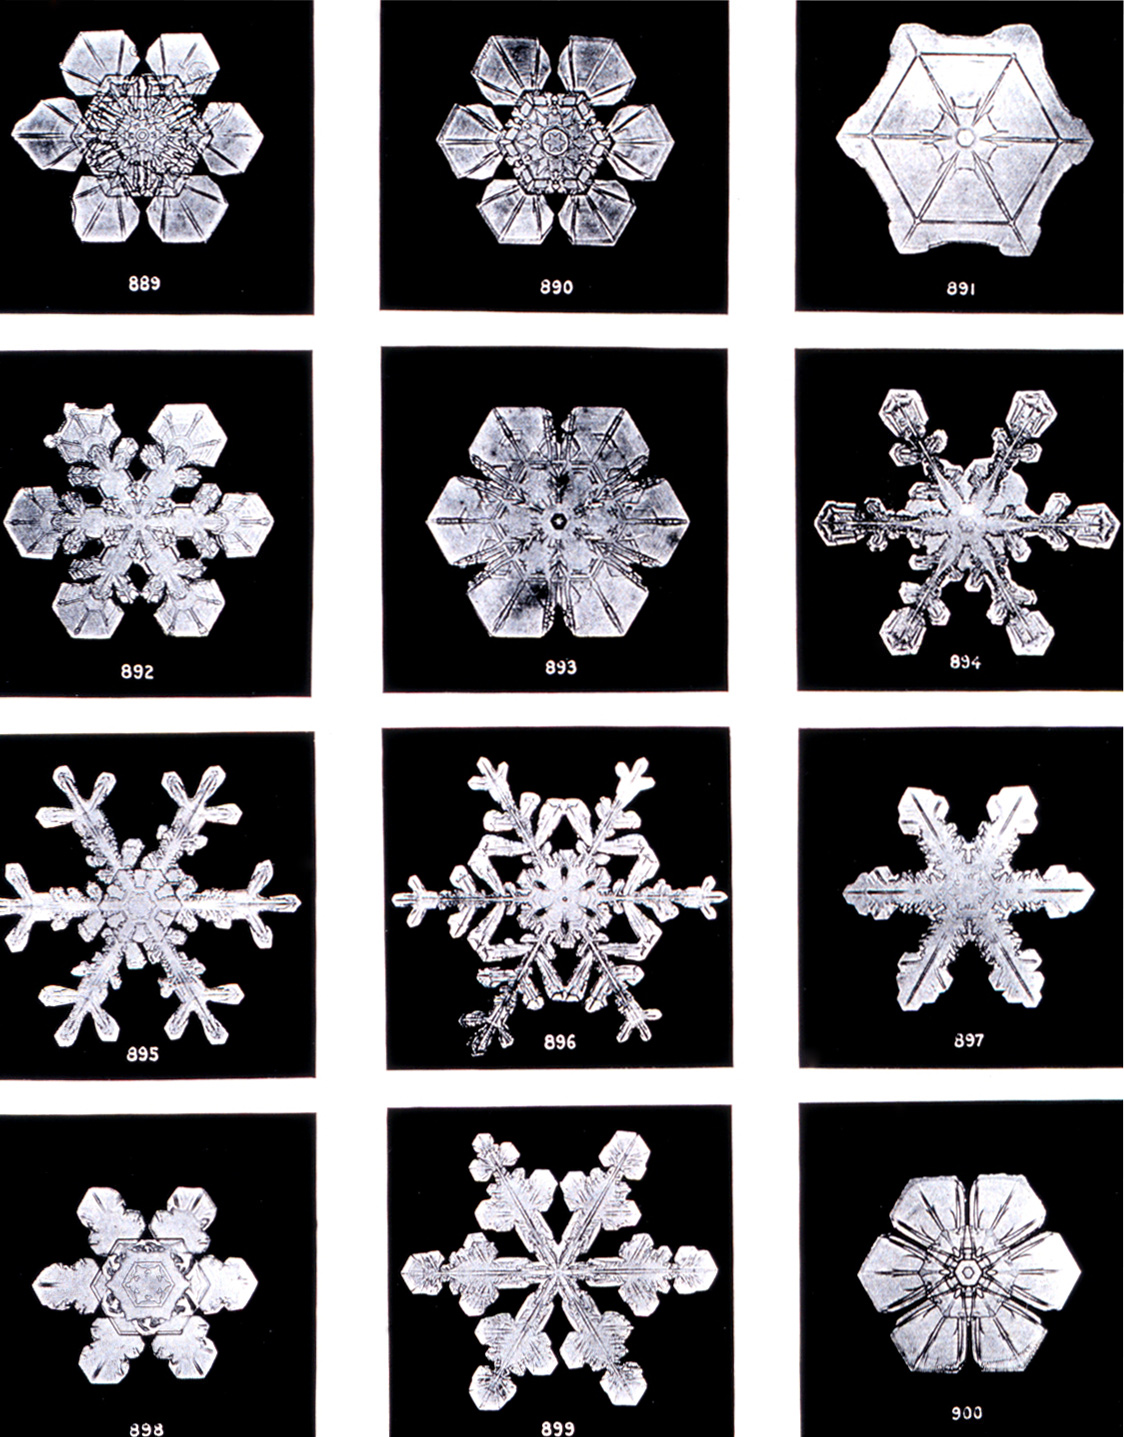
\includegraphics[width=0.36\linewidth]{images/book1/snowflakes.jpg}

{\small Cristais de neve fotografados por Wilson Bentley no começo do
século XX: todos têm seis ramos.}
\end{omfigure}

\section{Exercícios}


\begin{exercise}[$\star$]\label{exo:g11:polarity-and-cohesion:1}
Nas ligações \ce{H-Cl}, \ce{O-H} e \ce{C-O}, que \omterm{def:g7:atoms-and-molecules:atom}{átomo} tem a \omterm{def:g11:polarity-and-cohesion:polar-bond}{carga
parcial} $\delta^-$? Use a tabela de \omterm{def:g11:polarity-and-cohesion:electronegativity}{eletronegatividades}.
\end{exercise}

\begin{exercise}[$\star$]\label{exo:g11:polarity-and-cohesion:2}
Quais destas ligações são polares: \ce{H-H}, \ce{C-H}, \ce{O-H},
\ce{N-H}, \ce{Cl-Cl}, \ce{C-Cl}? Dê a diferença de \omterm{def:g11:polarity-and-cohesion:electronegativity}{eletronegatividades}
de cada uma.
\end{exercise}

\begin{exercise}[$\star$]\label{exo:g11:polarity-and-cohesion:3}
Que elemento é o mais eletronegativo em cada par: nitrogênio ou
fósforo; oxigênio ou enxofre; carbono ou nitrogênio; sódio ou magnésio?
Que tendência da tabela cada par ilustra?
\end{exercise}

\begin{exercise}[$\star$]\label{exo:g11:polarity-and-cohesion:4}
Quais de \ce{CH4}, \ce{NH3}, \ce{H2O} e \ce{HCl} podem formar \omterm{def:g11:polarity-and-cohesion:hydrogen-bond}{ligações
de hidrogênio} entre as suas próprias \omterm{def:g7:atoms-and-molecules:molecule}{moléculas}? Explique.
\end{exercise}

\begin{exercise}[$\star$]\label{exo:g11:polarity-and-cohesion:5}
Existem atrações entre as \omterm{def:g11:polarity-and-cohesion:polar-molecule}{moléculas apolares} do metano? Por que, mesmo
assim, o metano é um gás à temperatura ambiente?
\end{exercise}

\begin{exercise}[$\star\star$]\label{exo:g11:polarity-and-cohesion:6}
Diga se cada \omterm{def:g7:atoms-and-molecules:molecule}{molécula} é polar: diclorometano \ce{CH2Cl2} (tetraédrica),
tetraclorometano \ce{CCl4}, amônia \ce{NH3}, dióxido de carbono
\ce{CO2}, trifluoreto de boro \ce{BF3} (um triângulo plano com o boro no
centro).
\end{exercise}

\begin{exercise}[$\star\star$]\label{exo:g11:polarity-and-cohesion:7}
No metanol, \ce{CH3-OH}, que \omterm{def:g7:atoms-and-molecules:atom}{átomo} de hidrogênio pode ser doado numa
\omterm{def:g11:polarity-and-cohesion:hydrogen-bond}{ligação de hidrogênio}? Que \omterm{def:g7:atoms-and-molecules:atom}{átomo} pode receber uma? As \omterm{def:g7:atoms-and-molecules:molecule}{moléculas} de
metanol e de água podem formar \omterm{def:g11:polarity-and-cohesion:hydrogen-bond}{ligações de hidrogênio} entre si? Desenhe
uma.
\end{exercise}

\begin{exercise}[$\star\star$]\label{exo:g11:polarity-and-cohesion:8}
Explique por que as temperaturas de ebulição sobem na ordem \ce{CH4} <
\ce{SiH4} < \ce{GeH4}.
\end{exercise}

\begin{exercise}[$\star\star$]\label{exo:g11:polarity-and-cohesion:9}
No gráfico das temperaturas de ebulição dos hidretos, que grupo não
mostra nenhum valor anormal para o seu primeiro membro? Por quê?
\end{exercise}

\begin{exercise}[$\star\star$]\label{exo:g11:polarity-and-cohesion:10}
% ledger: en:H, en:Cl, en:Br, en:I, bp:HCl, bp:HBr, bp:HI
As ligações \ce{H-Cl}, \ce{H-Br}, \ce{H-I} são cada vez menos polares
(as \omterm{def:g11:polarity-and-cohesion:electronegativity}{eletronegatividades} do cloro, do bromo e do iodo são 3.16, 2.96 e
2.66), mas as temperaturas de ebulição sobem: \qty{-85}{\celsius},
\qty{-66}{\celsius}, \qty{-35}{\celsius}. Que interação vence, e por
quê?
\end{exercise}

\begin{exercise}[$\star\star$]\label{exo:g11:polarity-and-cohesion:11}
À temperatura ambiente, o cloro é um gás e o iodo um sólido, embora os
dois sejam formados por \omterm{def:g11:polarity-and-cohesion:polar-molecule}{moléculas apolares} \ce{X2}. Explique.
\end{exercise}

\begin{exercise}[$\star\star\star$]\label{exo:g11:polarity-and-cohesion:12}
% ledger: bp:C2H5OH, bp:CH3OCH3, bp:C3H8
O etanol \ce{CH3-CH2-OH}, o metoximetano \ce{CH3-O-CH3} e o propano
\ce{CH3-CH2-CH3} têm quase a mesma \omterm{def:g10:the-mole:molar-mass}{massa molar}. Eles fervem a
\qty{78}{\celsius}, \qty{-25}{\celsius} e \qty{-42}{\celsius}. Quais
deles são polares? Quais formam \omterm{def:g11:polarity-and-cohesion:hydrogen-bond}{ligações de hidrogênio} entre as suas
próprias \omterm{def:g7:atoms-and-molecules:molecule}{moléculas}? Explique a ordem.
\end{exercise}

\begin{exercise}[$\star\star\star$]\label{exo:g11:polarity-and-cohesion:13}
No gelo, cada \omterm{def:g7:atoms-and-molecules:molecule}{molécula} de água está ligada por \omterm{def:g11:polarity-and-cohesion:hydrogen-bond}{ligações de hidrogênio} a
quatro vizinhas, numa rede aberta; na água líquida, a rede se rompe o
tempo todo e desaba em parte. Explique por que o gelo flutua na água.
Por que isso é importante para os peixes de um lago congelado?
\end{exercise}

\begin{exercise}[$\star\star\star$]\label{exo:g11:polarity-and-cohesion:14}
Ordene por temperatura de fusão crescente, e justifique pelas atrações
entre as partículas: cloreto de potássio \ce{KCl}, gelo \ce{H2O}, metano
sólido \ce{CH4}.
\end{exercise}

\begin{exercise}[$\star\star\star$]\label{exo:g11:polarity-and-cohesion:15}
% ledger: en:F, en:O, bp:HF, bp:H2O
O flúor é mais eletronegativo que o oxigênio, por isso uma ligação
\ce{H-F} é mais polar que uma ligação \ce{O-H}. Mesmo assim, a água ferve
a \qty{100}{\celsius} e o fluoreto de hidrogênio a \qty{20}{\celsius}.
Conte os \omterm{def:g7:atoms-and-molecules:atom}{átomos} de hidrogênio que cada \omterm{def:g7:atoms-and-molecules:molecule}{molécula} pode doar e os \omterm{def:g10:lewis-and-shape:lone-pair}{pares não
ligantes} com que ela pode receber, e explique.
\end{exercise}

\section{Problema: por que a água ferve a \texorpdfstring{\qty{100}{\celsius}}{100 graus Celsius}?}

\begin{problem}[{Problema de fim de semana --- sem ligações de
hidrogênio, a que temperatura a água ferveria?}]
\label{pb:g11:polarity-and-cohesion:1}
% ledger: en:H, en:O, en:S, en:Se, bp:H2O, bp:H2S, bp:H2Se, bp:CH4, bp:SiH4, bp:GeH4, bp:HCl, bp:HBr, bp:HF, bp:NH3, bp:PH3, bp:AsH3
O oxigênio, o enxofre e o selênio estão no mesmo grupo da tabela, e os
três formam um composto com o hidrogênio: \ce{H2O}, \ce{H2S}, \ce{H2Se}.
Em cada grupo de hidretos, as temperaturas de ebulição em geral sobem
com o tamanho da \omterm{def:g7:atoms-and-molecules:molecule}{molécula}. A água quebra a regra. Em quanto?

\medskip
\noindent\textbf{Parte I --- Três \omterm{def:g7:atoms-and-molecules:molecule}{moléculas}.}
\begin{enumerate}
  \item Desenhe as \omterm{def:g10:lewis-and-shape:lewis-structure}{estruturas de Lewis} de \ce{H2O}, \ce{H2S} e
        \ce{H2Se}. Por que elas se parecem?
  \item Calcule as suas \omterm{def:g10:the-mole:molar-mass}{massas molares}.
  \item Calcule as diferenças de \omterm{def:g11:polarity-and-cohesion:electronegativity}{eletronegatividade} das ligações
        \ce{O-H}, \ce{S-H} e \ce{Se-H} (oxigênio 3.44, enxofre 2.58,
        selênio 2.55, hidrogênio 2.20). Que ligações são claramente
        polares?
  \item Qual é a geometria das três \omterm{def:g7:atoms-and-molecules:molecule}{moléculas}? Elas são polares?
  \item Conte os \omterm{def:g9:inside-the-atom:nucleus}{elétrons} de cada \omterm{def:g7:atoms-and-molecules:molecule}{molécula}. Qual tem as \omterm{def:g11:polarity-and-cohesion:van-der-waals}{interações de
        van der Waals} mais fortes?
\end{enumerate}

\medskip
\noindent\textbf{Parte II --- As \omterm{def:g11:polarity-and-cohesion:hydrogen-bond}{ligações de hidrogênio}.}
\begin{enumerate}[resume]
  \item Qual dos três compostos forma \omterm{def:g11:polarity-and-cohesion:hydrogen-bond}{ligações de hidrogênio} entre as
        suas \omterm{def:g7:atoms-and-molecules:molecule}{moléculas}? Por que não os outros?
  \item De quantas \omterm{def:g11:polarity-and-cohesion:hydrogen-bond}{ligações de hidrogênio} uma \omterm{def:g7:atoms-and-molecules:molecule}{molécula} de água pode
        participar, no máximo? Desenhe-as.
  \item Que interações mantêm as \omterm{def:g7:atoms-and-molecules:molecule}{moléculas} de sulfeto de hidrogênio
        juntas no líquido?
\end{enumerate}

\medskip
\noindent\textbf{Parte III --- A tendência.}
\begin{enumerate}[resume]
  \item O sulfeto de hidrogênio ferve a \qty{212.9}{K} e o seleneto de
        hidrogênio a \qty{-41.3}{\celsius}. Expresse a primeira em graus
        Celsius ($\theta = T - 273.15$).
  \item Em quanto a temperatura de ebulição sobe do período 3
        (\ce{H2S}) para o período 4 (\ce{H2Se})?
  \item Por que ela sobe?
  \item Supondo a mesma subida do período 2 para o período 3, a que
        temperatura ferveria uma \ce{H2O} ``normal''?
  \item Teste o método no \omterm{def:g9:periodic-table-first-look:period}{grupo} 14: o \ce{SiH4} ferve a
        \qty{-112}{\celsius} e o \ce{GeH4} a \qty{-88.1}{\celsius}.
        Preveja a temperatura de ebulição do \ce{CH4} e compare com a
        real, \qty{-162}{\celsius}. A extrapolação é exata?
  \item Faça o mesmo para o \omterm{def:g9:periodic-table-first-look:period}{grupo} 17 (\ce{HCl} \qty{-85.1}{\celsius},
        \ce{HBr} \qty{-66.4}{\celsius}) e compare com o \ce{HF},
        \qty{19.6}{\celsius}.
\end{enumerate}

\medskip
\noindent\textbf{Parte IV --- A diferença.}
\begin{enumerate}[resume]
  \item A água ferve de verdade a \qty{100}{\celsius}. Qual é o tamanho
        da diferença entre o valor real e o valor extrapolado?
  \item O mesmo para a amônia, usando \ce{PH3} \qty{-87.8}{\celsius} e
        \ce{AsH3} \qty{-62.5}{\celsius}; a amônia ferve de verdade a
        \qty{-33.4}{\celsius}.
  \item Ordene a água, o fluoreto de hidrogênio e a amônia pelo tamanho
        da sua diferença, e explique a ordem contando as \omterm{def:g11:polarity-and-cohesion:hydrogen-bond}{ligações de
        hidrogênio}.
  \item Sem \omterm{def:g11:polarity-and-cohesion:hydrogen-bond}{ligações de hidrogênio}, a água seria um sólido, um líquido ou
        um gás à temperatura ambiente? O que isso significaria para a
        Terra?
  \item Por que a resposta da questão 12 é só uma estimativa?
  \item Dê a resposta final: a cerca de que temperatura a água ferveria
        sem \omterm{def:g11:polarity-and-cohesion:hydrogen-bond}{ligações de hidrogênio}?
\end{enumerate}
\end{problem}
